\documentclass[aspectratio=169,10pt]{beamer}
\usepackage{fontspec}
\usepackage{polyglossia}
\setdefaultlanguage{russian}
\setotherlanguage{english}
\setmainfont{DejaVu Sans}
\usepackage{graphicx}
\setsansfont{DejaVu Sans}
\setmonofont{DejaVu Sans Mono}
\definecolor{teal}{HTML}{0A685B}
\definecolor{dark}{HTML}{153B35}
\definecolor{pale}{HTML}{E8F4EE}
\definecolor{orange}{HTML}{A95A33}
\setbeamercolor{frametitle}{fg=dark}
\setbeamercolor{title}{fg=dark}
\setbeamercolor{structure}{fg=teal}
\setbeamercolor{block title}{bg=teal,fg=white}
\setbeamercolor{block body}{bg=pale,fg=dark}
\setbeamercolor{block title alerted}{bg=orange,fg=white}
\setbeamercolor{block body alerted}{bg=orange!9,fg=dark}
\setbeamertemplate{navigation symbols}{}
\setbeamertemplate{footline}{\hfill\scriptsize\insertframenumber\, / \,\inserttotalframenumber\hspace{12pt}\vspace{5pt}}
\setbeamertemplate{itemize item}{\raisebox{.2ex}{\tiny$\blacktriangleright$}}
\setbeamerfont{frametitle}{size=\Large,series=\bfseries}
\setbeamerfont{normal text}{size=\normalsize}
\setlength{\leftmargini}{1.3em}
\begin{document}
\begin{frame}[plain]
\begin{beamercolorbox}[wd=\paperwidth,ht=\paperheight,sep=1.4cm,center]{title}
\vspace*{1.0cm}{\large Данные как основа ИИ · семестр 2}\par\vspace{1cm}
{\fontsize{30}{38}\selectfont\bfseries Связь видна. Причина — нет}\par\vspace{0.6cm}
{\large Корреляция, группы и аналитические выводы}\par\vfill{\small Кейс «Умный кампус» · университетские пространства}
\end{beamercolorbox}\end{frame}
\begin{frame}[t]{Парадокс первой корреляции}
\vspace{.15cm}\begin{itemize}
\item 108 сессий: число людей и CO₂.\vspace{6pt}
\item Общий коэффициент корреляции отрицателен.\vspace{6pt}
\item Это означает, что присутствие людей уменьшает CO₂?\vspace{6pt}
\end{itemize}
\vfill\begin{alertblock}{Вопрос аудитории}\large Почему нет?\end{alertblock}
\end{frame}
\begin{frame}[t]{Единица наблюдения важнее числа строк}
\vspace{.15cm}\begin{itemize}
\item Одна строка = одна сессия, не один студент.\vspace{6pt}
\item В данных несколько помещений и режимов вентиляции.\vspace{6pt}
\item Прежде чем объединять, нужно понять, что сравнивается.\vspace{6pt}
\end{itemize}
\end{frame}
\begin{frame}[t]{Сначала диаграмма рассеяния}
\vspace{.15cm}\begin{itemize}
\item Каждая точка соответствует двум числовым значениям.\vspace{6pt}
\item По расположению точек видны тренды, группы и нелинейность.\vspace{6pt}
\item Числовой коэффициент — дополнение, не замена графику.\vspace{6pt}
\end{itemize}
\end{frame}
\begin{frame}[t]{Знак корреляции}
\vspace{.15cm}\begin{itemize}
\item Положительная линейная связь: X и Y чаще растут вместе.\vspace{6pt}
\item Отрицательная: при большем X чаще наблюдается меньший Y.\vspace{6pt}
\item Нулевой r не исключает нелинейные зависимости.\vspace{6pt}
\end{itemize}
\end{frame}
\begin{frame}[t]{Две группы меняют вывод}
\vspace{.15cm}\begin{itemize}
\item Совместно наблюдения дают отрицательную корреляцию.\vspace{6pt}
\item Внутри каждого режима вентиляции — положительную.\vspace{6pt}
\item Нужно изучить различия групп и условия отбора.\vspace{6pt}
\end{itemize}
\end{frame}
\begin{frame}[t]{Что видно на данных?}
\vspace{.4cm}
\centering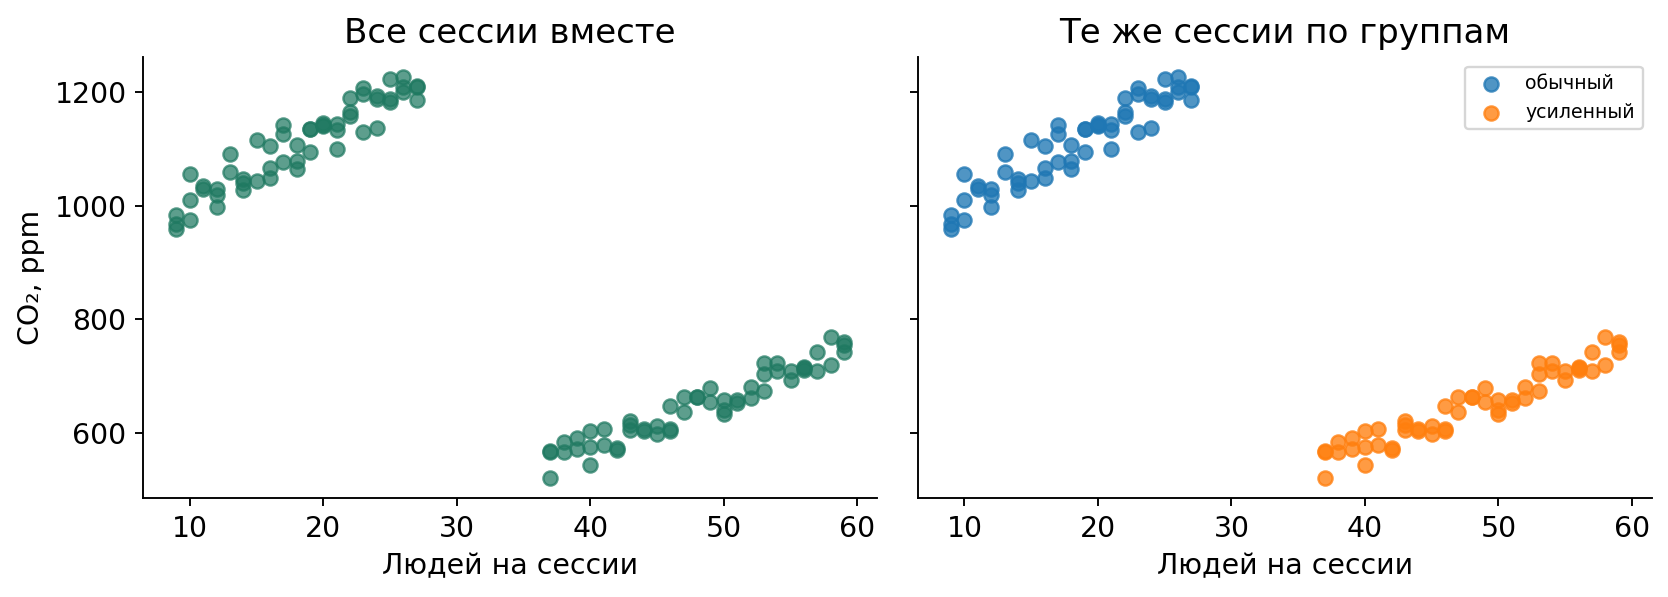
\includegraphics[width=.94\linewidth]{../assets/chart07_groups.png}
\end{frame}
\begin{frame}[t]{Почему так происходит?}
\vspace{.15cm}\begin{itemize}
\item Обычный режим: меньшие помещения и более высокие CO₂.\vspace{6pt}
\item Усиленный: большие помещения, больше людей, ниже CO₂.\vspace{6pt}
\item Эти различия влияют на общую картину.\vspace{6pt}
\end{itemize}
\end{frame}
\begin{frame}[t]{Что такое смешение}
\vspace{.15cm}\begin{itemize}
\item Третий фактор связан с X и с Y.\vspace{6pt}
\item В объединённых данных коэффициент отражает несколько процессов.\vspace{6pt}
\item Разбиение по группам помогает увидеть структуру, но не доказывает причину.\vspace{6pt}
\end{itemize}
\end{frame}
\begin{frame}[t]{Факт, гипотеза, проверка}
\vspace{.15cm}\begin{itemize}
\item Факт: в данных внутри режимов корреляция положительна.\vspace{6pt}
\item Гипотеза: при сопоставимых условиях рост посещаемости влияет на CO₂.\vspace{6pt}
\item Проверка: собрать сравнимые условия и дополнительные измерения.\vspace{6pt}
\end{itemize}
\end{frame}
\begin{frame}[t]{Корреляция не равна причинности}
\vspace{.15cm}\begin{itemize}
\item Для причинного вывода нужны аргументы о механизме и альтернативных объяснениях.\vspace{6pt}
\item Даже очень большой |r| не является экспериментом.\vspace{6pt}
\item Не делаем управленческие рекомендации из одного коэффициента.\vspace{6pt}
\end{itemize}
\end{frame}
\begin{frame}[t]{А что с проверкой гипотез?}
\vspace{.15cm}\begin{itemize}
\item Сначала вопрос, единица наблюдения и сопоставимые группы.\vspace{6pt}
\item Лишь потом выбирают статистический метод.\vspace{6pt}
\item «Значимо» не равно «важно» и не появляется без вычисления.\vspace{6pt}
\end{itemize}
\end{frame}
\begin{frame}[t]{ИИ как редактор вывода}
\vspace{.15cm}\begin{itemize}
\item Модель может рассчитать r и предложить версии объяснений.\vspace{6pt}
\item Попросите отделить расчёт, гипотезу и рекомендации.\vspace{6pt}
\item Все объяснения сверяем с данными и условиями их получения.\vspace{6pt}
\end{itemize}
\end{frame}
\begin{frame}[t]{Разные маршруты, одна компетенция}
\vspace{.15cm}\begin{itemize}
\item Таблицы: общий и групповые коэффициенты, диаграммы.\vspace{6pt}
\item Python: воспроизводимый разрез, программные проверки.\vspace{6pt}
\item Исследование: смешивающие факторы и план проверки.\vspace{6pt}
\end{itemize}
\end{frame}
\begin{frame}[t]{Выходной билет}
\vspace{.15cm}\begin{itemize}
\item Почему знак общего r отличается от внутригруппового?\vspace{6pt}
\item Что ещё отличается между группами?\vspace{6pt}
\item Как переформулировать причинный вывод как наблюдение?\vspace{6pt}
\end{itemize}
\end{frame}
\end{document}